\section{Implementation}
\label{sec:implementation}
The prototype is tailored to a smaller scale of a home environment. It has features to control and monitor the power consumption from each device included in the background load, which, in our data set, corresponds to a fridge and a floor heater. We also gain data from the total power consumption, where interactive load is included. The implemented and evaluated algorithm to the problem with peak avoidance is based on the one found in \cite{barker2012smartcap}.

\subsection{Test Data}
At this stage we do not have a real home environment to run our system in and we have therefore acquired 24 hours of test data from a real home in Sweden and fed it to our system through an \emph{SQLite} database. Since the behaviour of the background loads will be altered in our system, their normal behaviour must be analyzed in order to estimate how long the respective load can be powered down before they must be powered up again and vice versa. 

In figure \ref{PowerTrace} the consumption trace of the fridge and the floor heater from the database is illustrated. Since the test data is not that fine grained (10 minutes interval) the analysis of the behaviour is only approximate. It is concluded that this fridge, which typically operates in temperatures between four to six degrees, can be powered down for approximately 20 minutes before the temperature reaches the upper bound if it begins at the lowest temperature. It then needs to be powered for 80 minutes before reaching the lower bound again. When powered, the fridge consumes about 16 watts in average. It should also be noted that if the fridge door is opened, the temperature will rise much faster and the fridge will need power sooner than predicted. This phenomenon however, has not been clearly noticed in the test data from the fridge and is therefore neglected in our simulation, but would automatically be taken into account in a real-life scenario.

The floor heater can have much longer down time. It can be powered down for 30 minutes before the temperature reaches its lower bound and then needs to be powered for 10 minutes. Thus, the floor heater also requires much less on-time than the fridge, but on the other hand, the consumption of the floor heater, when powered up, is 80 watts during most hours, but with a severe peak in the afternoon with a consumption of a staggering 180 watts. There are a few possible explanations for this peak. It could be that the floor heater is on a timer that will increase the temperature just before the occupants get back home from work. It could also be that the occupants get home on a winter day and brings snow inside. The temperature on the floor will then drop and extra power is needed to satisfy the set temperature bounds. The reason is not important, but the extra consumption of the floor heater during certain hours is considered in our scheduler.


\begin{figure}[!h]
\centering
    \begin{subfigure}[b]{0.52\textwidth}
            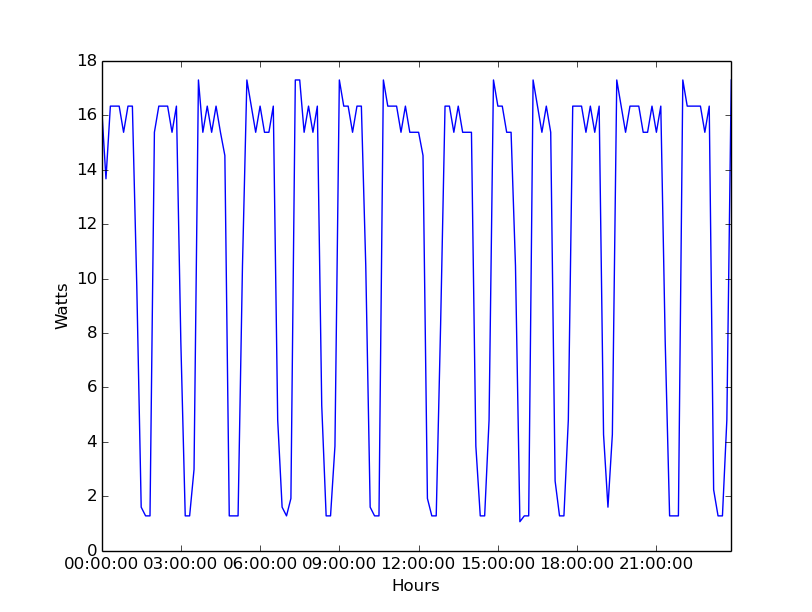
\includegraphics[width=\textwidth]{img/fridge.png}
            \caption[Peaks]{\emph{\small Fridge.}}
            \label{fig:fridgePowerTrace}
        \end{subfigure}%
        ~
        \begin{subfigure}[b]{0.52\textwidth}
            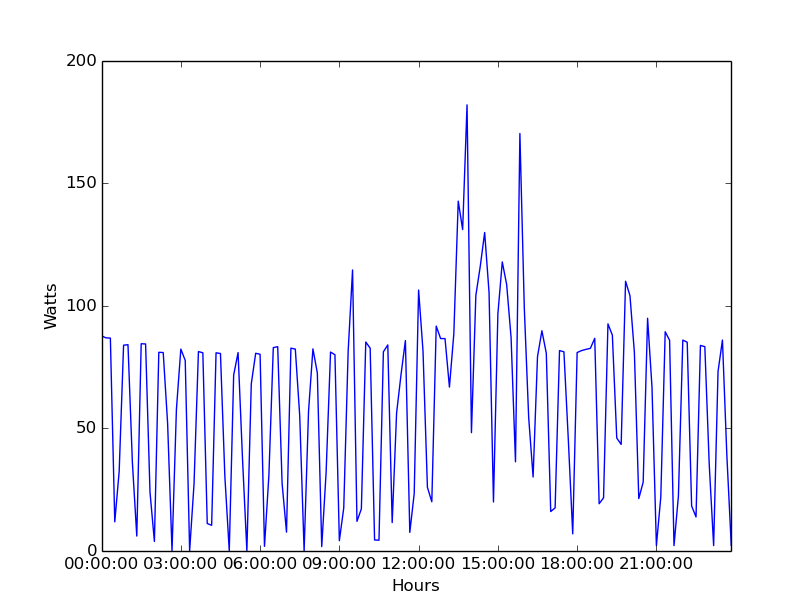
\includegraphics[width=\textwidth]{img/floor_heating.png}
            \caption[Peaks]{\emph{\small Floor heater.}}
            \label{fig:floorHeaterPowerTrace}
        \end{subfigure}%
\caption[Peaks]{\emph{\small Consumption trace of background loads.}}
\label{PowerTrace}
\end{figure}

\subsection{Least Slack First (LSF)}

Likewise the article by Baker et al. we use the \emph{Least Slack First} (LSF) algorithm to schedule devices that represent the background load. It should be noted that the LSF algorithm is inspired by the well known earliest deadline first algorithm used in real-time operating systems \cite{barker2012smartcap}. 

In the algorithm there is a consumption threshold that ensures we do not power up too many appliances at the same time. The algorithm sums the total consumption of all active interactive loads and then power background loads until the total load crosses the threshold. The threshold, in our solution, is a calculated average of the last hour's consumption. Choosing such an average will make the threshold follow the natural shift in power demand during different hours of the day. If some background load has slack zero it will, if necessary, breach the threshold since this load must have power. The difference between our solution and the one presented by Barker et al. is that we also consider the interactive loads when calculating the threshold and when scheduling the background loads. This means that our solution could take action and power down all background loads if there is a high peak in the interactive loads in order to prevent the highest peaks. 

For the solution to be attractive and possible to implement in homes, it must not require a change of habits of the occupants. Therefore, all bounds discussed in the previous section must be held and no interactive load can be controlled from the system. In this report we define slack as the measure of how long a background load can remain off without affecting its bound, e.g. the temperature in the fridge. The device that has the least slack will have priority over the others. If the slack reaches zero for some device, the device is forced to start, no matter what the current load from other devices is.

\subsection{System Description}
The system consists of a scheduler developed in Python. The scheduler in turn communicates with an \emph{SQLite} database which holds test data for a 24-hour period. The nodes are built with the help of an off-the-shelf system called \emph{Plugwise} \cite{plugwise2014}. \emph{Plugwise} handles the communication between devices in the home using a wireless \emph{Zigbee} meshed network. Since \emph{Plugwise} does not offer any open API we have used a third-party library to communicate with the nodes \cite{hadaraplugwise}. The hardware we used belong to the product \emph{Plugwise} and consists of two power switches, which are controlled from our computer by a USB wireless adapter.

The prototype consists of one coordinator thread and then one thread for each background load. The background threads monitor the slack of each device and also turn the power to the device on and off. The coordinator thread monitors the current consumption from the interactive loads and together with the reported slack from the background threads makes the scheduling decisions and orders the background threads to power their device on or off.

While running the simulation we plot the result dynamically, showing the difference in real-time. In figure \ref{runView} we illustrate our system. In the picture we have a fridge and an air conditioner (in the simulation the AC is replaced with a floor heater). We also have a third variable, the interactive loads (television, radio, computer, coffee maker), which will affect the other two when started, but cannot be controlled by the system.

\begin{figure}[!ht]
\centering
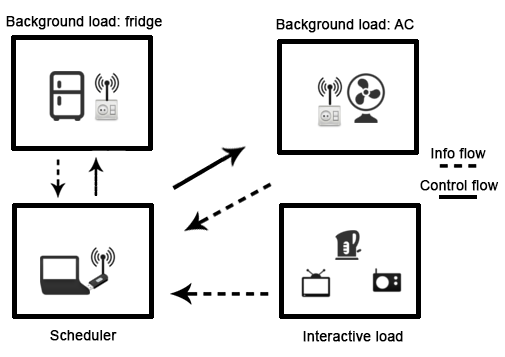
\includegraphics[width=0.75\textwidth]{img/dat300_final_desc.png}
\caption[Project Description]{\emph{\small Description of the implemented system.}}
\label{runView}
\end{figure}

%% Korrekturläst av Anders 2014-12-03